\documentclass{report}

\usepackage{graphicx}
\usepackage{float}
\usepackage{hyperref}

\setlength\parindent{0pt}

%----------------------------------------------------------------------------------------
%	DOCUMENT INFORMATION
%----------------------------------------------------------------------------------------

\title{Exercise 1 \\ Pipelined MIPS \\ TDT4255} % Title

\author{Hanna Holler Kamperud \\ Olav Emil Eiksund \\ Christian Chavez} % Author name

\date{\today} % Date on the report

\begin{document}

\maketitle % Insert the title, author and date

\newpage
\begin{abstract}
\begin{abstract}
After the proliferative growth of complexity anticipated by Moore's law, the
processor technology has had to struggle more and more in finding ways to
increase throughput without hitting their many limitations due to their
complexity. Pipelining is a technique to utilize the components in a processor
much more efficiently, by reducing downtime as much as possible. This through
identifiying seperable stages which can work independently of each other, and
segregating these so that (under ideal circumstances) no stage in the pipeline
has any inactive circuits at any given time.
\paragraph*{}
This technique has been implemented successfully throughout the industry, and
there are mainstream processors on the market without pipelining to this day.
\paragraph*{}
In this assignment, the goal has been to produce a five-stage pipelined MIPS
processor. This has been realized through current industry tools such as
Xilinx's Integrated Software Environment Project Navigator and Platform Studio,
which are both part of the Xilinx Design Suite \cite{xilinx-ise}
\paragraph*{}
The goal of this assignment has been for us students to learn how pipelined
processors work, and to gain familiarity with the current industry tools used
for the design of such processors, by way of implementing it on an embedded
device containing an FPGA chip, the Xilinx Spartan-6 \cite{spartan-6}.
\paragraph*{}
For this assignment, the suggestions in the book \cite{patterson12}, the Course
\cite{course} lectures and slides, and the Compendium \cite{compendium}.
\end{abstract}

\end{abstract}

\tableofcontents
%\listoffigures

%----------------------------------------------------------------------------------------
%	INTRODUCTION
%----------------------------------------------------------------------------------------

\chapter{Introduction}
\section{Description of the exercise}

\subsection{Description introduction}

In this second assignment, we have extended the processor from the previous
assignment by changing the datapath into a pipeline. This had the consequence
that pipelines had to be added to the design, as well as write a new control
module to support the pipeline processing.
\paragraph*{}
Additionally, we have
implemented a hazard detection unit and a forwarding unit to guard the
processor from hazards by using correction techniques. The forwarding unit
sends data yet to be written to memory to previous pipeline stages where later
instructions need the current values. The hazard detection unit inserts
``bubbles'' into the pipeline, stalling a selected stage for the duration of a
pipeline clockcycle. It does this to stop a new instruction reading from a
register which a previous instruction is currently writing to.
\paragraph*{}
Both these units have but one intention and consequence, and that is
implementing a more efficient design of the pipelined processor by avoiding
stalls and hazards.

\subsection{Assignment requirements}
\emph{The below text has been copied from the Course Compendium
\cite{compendium}.}\newline
``The major requirement of this assignment is a simple 5-stage pipelined
processor. In general, the processor has the same functional requirements as in
the previous assignment. Additionally, you need to implement different hazard
detection and correction techniques. You will also use the same test set up. To
help you on the way, we have made a suggestion from which you can work on. It is
wise to make a processor which relies on the design from the previous assignment
so that you can reuse the test benches and test programs.''
\paragraph*{}
In consequence, we interpreted this to mean that we needed the following:
\begin{enumerate}
	\item To design a pipelined processor.
	\begin{enumerate}
		\item With five pipeline stages.
	\end{enumerate}
	\item The processors functionality will be based on the functionality of a
``MIPS'' processor.
	\item A Forwarding unit to deal with some of the hazards a pipelined
processor brings.
	\item A Hazard Detection unit to deal with the hazards that occur when a
processor reads and writes in two different pipeline stages.
\end{enumerate}


\section{Approach to the task}
Our approach to the task has been an iterative approach. Slide 58 on the
\emph{Pipelining} \cite{slides-6} course lecture illustrates a pipelined design
whose components resemble the previous assignment in this course very closely.
Due to this, we decided to start by converting the functioning processor design
from the previous assignment into a pipelined processor based on the design on
the abovementioned diagram. The diagram is taken from the book
\cite{patterson12}, on page 362.
\paragraph*{}
Following the approach of the authors through the chapters of the book, we had
few problems implementing the first version of our processor design, and
continued to work towards a more complex design including hazard controls by way
of forwarding and stalling. Slide 57 from lecture \cite{slides-7} illustrates
the functional architecture of our final processor design. This design builds
upon the previous one with several improvements, which include the forwarding
unit and the hazard control unit.
\paragraph*{}
Finally, when the design was completed, we tested it out in the lab to discover
any errors not previously found in our design (and subsequently fixing them).

%----------------------------------------------------------------------------------------
%	SOLUTION
%----------------------------------------------------------------------------------------

%\newpage
\chapter{Solution}

%ISA

\section{Design}
\section{Design}
The design is based on, and almost equivalent with the design described in the
book. The focus of this section is to highlight and explain the differences
between the two, rather than describing it in detail. For further details on the
design see \cite{patterson12}.
\subsection{Memory address space}
Since the memory is synthesized with $2^8$ addresses, constants were redefined
throughout the project to reflect this, thus avoiding a large number of
synthesize warnings regarding unused address bits. The only functional change
this implies is a simplification of the jump instruction, where it only needs
the eight least significant bits of the immediate value. Given that this design
is to be implemented on an FPGA, it seems reasonable to reduce the address
space from 512 MiB to 256 bit.

\subsection{Pipeline registers}
Since the DMEM, IMEM and register file components synthesize into block ram, the
need for additional pipeline registers storing these values dissappear.
Including these would introduce a delay in the propagation of the corresponding
signals. These registers have therefore been removed, and some steps had to be
taken to maintain equal functionality. For instance, the flushing of the IF/ID
instruction register has to happen dynamically, in a VHDL-process operating on
the instruction data signal from stage 1.

\subsection{Other}
\textbf{TO DO!!!!!}


\section{Implementation}
Similarly to the last exercise, a hierarchical structure was used where the
processor had each stage as a component. This was done to provide abstraction,
as well as simplifying the implementation.
\paragraph*{}
The VHDL component called \emph{pipeline\_stage1} consists of the abstracted
pipeline stages 0 and 1, since each of these are relatively small in their own
right. Stage 2 was mostly implemented how it was designed, but the hazard
detection unit and control unit were placed inside this stage. This was done
since most signals connecting to these units go to stage 2.
\paragraph*{}
Stage 5 did not get its own VHDL component, since the program counter was
written into the stage 1 component. The rest of the stage 5 logic fit better
inside the processor component. The forwarding unit was placed as a component in the
processor file to avoid further complexity in the VHDL components.

\subsection{Processor core}
The processor core itself was implemented as a messenger between the pipeline
stages, similarly to how toplevel works with respect to the core, com and mem
units.
\paragraph*{}
To make it obvious where a signal came from each was prefixed with
``\emph{stage\_\#\_out\_}'', since many of the signals had the same name in
different stages. In addition, all component definitions and port maps were
grouped and documented according to where they were connected, making it easy to
locate a desired signal. These steps helped a great deal during development, but
may have been neglected during testing/bugfixing.
\paragraph*{}
Since it was unclear whether memory access would consume a processing cycle or
 need a pipeline register, IMEM was connected directly to stage one, and
 instructions were then sent from a port in stage 1 onward to stage 2. This made
 it easy to implement or bypass the pipeline register as needed.
 
\subsection{Control unit}
The control unit was changed quite a lot from the previous assignment. Since it was used to control the multi-cycle functionality of the previous exercise, it could now be implemented without any states. Since it no longer needed to account for states, the control unit was reduced down to a compnent that no longer depended on the internal clock. A process inside the control unit responds to a change in the opcode and outputs the correct control signals for the new instruction. These new values are stored in the pipeline registers and propagated through the core. 

\subsection{Hazards}
We made an attempt at implementing hazard detection system such as (and
including) forwarding, stalling and flushing. The forwarding unit is based on
the description given in section 4.7 of \cite{patterson12}. Initially only the
forwarding unit given in the schematic was implemented, but recognizing the
need to forward values to the branch check after the register file, an
additional forwarding unit was instantiated.
\paragraph*{}
Dynamic branch prediction was postponed to give more time for testing, and
branches are in the design assumed to fall through. If this fails, the pipeline
is stalled, but the optimization of moving the branch check to stage 2 has been
implemented. Flushing the current instruction based on this branch value leads
to a combinatorial loop, and although it can probably be easily fixed, this
flushing was commented out during testing.
\paragraph*{}
A hazard detection unit also takes care of data hazards relating to reading
values from registers in use at the ALU stage (stage 3, RAW-hazards). The
hazard detection unit stalls the pipeline when the instruction passing from
stage 2 and into stage 3 involves a register read. If this is the case, and said
instruction reads from one of the two registers in use in stage 2, the unit will
enable the stall signal passing into stage 1. If the stall signal in stage 1 is
enables at clockcycle $n$, this has the consequence of all subsequent $n+1$
stages repeating their action at clockcycle $n+1$, creating an instruction
``bubble'' at stage $n+1$.


%----------------------------------------------------------------------------------------
%	RESULTS
%----------------------------------------------------------------------------------------
\newpage
\chapter{Results}
\input{results/intro}

\section{Testing methodology}
\subsection{First error found}
The first error we encountered when simulating our processor design in ModelSim
\cite{modelsim}, was an error where \emph{pipeline\_stage1} gives an undefined
value as output every second clockcycle.
\paragraph*{}
Figure \ref{fig:error-1-text} below illustrates the problem:
\begin{figure}[h]
	\caption{First error (you can view it fullscale in the appendix:
\ref{fig:error-1-landscape}).}
	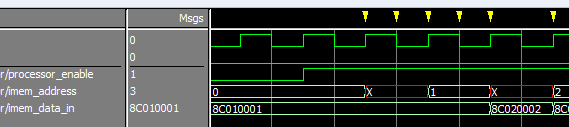
\includegraphics[scale=0.5]{figures/pc_error_annenhver_LITEN.png}
	\label{fig:error-1-text}
\end{figure}

\paragraph*{}
This problem was caused by the program counter's input in
\emph{pipeline\_stage1} not being properly connected to the adder incrementing
program counter's output. This problem was resolved by connecting the output
from the adder correctly into the multiplexor choosing between the adder and
branch values as inputs for the program counter.

\subsection{Second error found}
The second error encountered was when simulating the entire pipeline design as
a whole to check whether instructions as a whole propagated correctly.
\paragraph*{}
It was discovered (as figure \ref{fig:error-2-text} illustrates) that due to the
bottom signal ``stage\_4\_out\_wb'' being undeclared until the ALU operations unit
sends the load/store command to the ALU. The ``stage\_4\_out\_wb'' should not
have gotten the value 1 (logical high), before the signal ``alu\_mem\_mux\_out''
gets the value 2. Since it becomes logical high before this point, the
consequence is that garbage is written back to the registers in
\emph{pipeline\_stage2}.
\begin{figure}[H]
	\caption{Second error (you can view it fullscale in the appendix:
\ref{fig:error-2-landscape})}
	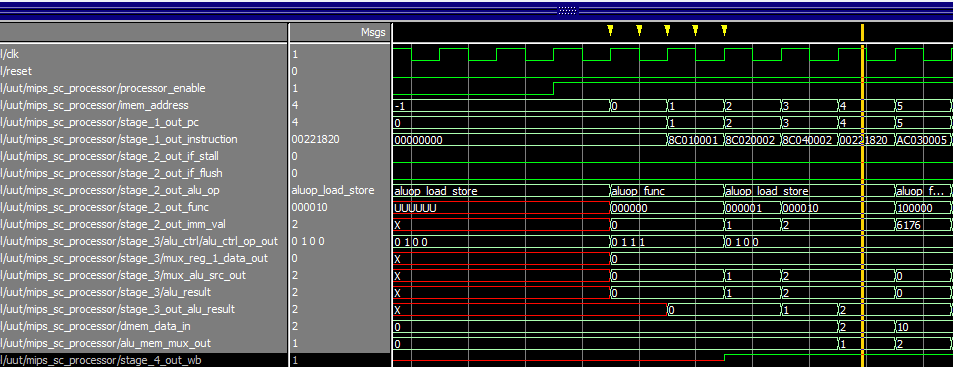
\includegraphics[scale=0.5]{figures/error_2.png}
	\label{fig:error-2-text}
\end{figure}

\paragraph*{}
This was never resolved. It was deemed to be a minor issue at first since it only occured during the first few cycles of the simulation. Then it was discovered that it was probably a symptom of a larger timing issue where the write back signal was set too early. There was also a correct value that only appeared for half a clock cycle before disappearing which was never written back to registers. This points to a larger timing issue which we were not able to resolve.

\subsection{First test}
\begin{figure}[H]
	\caption{First test. See also appendix section \ref{fig:test-1-landscape}).}
	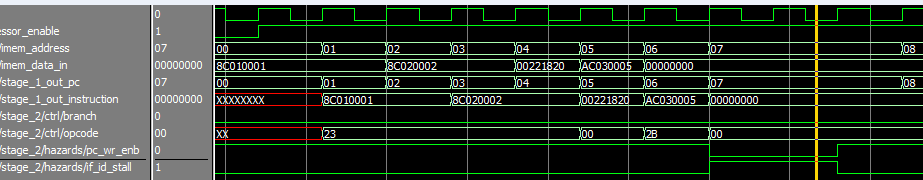
\includegraphics[scale=0.6]{figures/test_1_text.png}
	\label{fig:test-1-text}
\end{figure}

The first test we ran, as opposed to errors we encountered, was to test if the
stall functionality worked correctly with the program counter in \emph{
pipeline\_stage1}.
\paragraph*{}
Figure \ref{fig:test-1-text} illustrates how when the stall signal
``if\_id\_stall'' becomes one (logical high), the program counter's write-enable
signal ``pc\_wr\_enb'' turns off by becoming zero.
\paragraph*{}
The correct result of these actions are shown by the signals ``imem\_address''
and ``stage\_1\_out\_pc''. You can see that before the stall signal turns on,
these two aforementioned signal values increment on each clock cycle. Yet when
the stall signals turns on, they keep their value, and only continue
incrementing after it stall has been turned off again by reverting to zero.


\section{fpga}
The design was never tested on the FPGA. For more detailes refer to the the Discussion chapter.

%----------------------------------------------------------------------------------------
%	DISCUSSION
%----------------------------------------------------------------------------------------
\newpage
\chapter{Discussion}
\section{Design}
\section{Design}
The design is based on, and almost equivalent with the design described in the
book. The focus of this section is to highlight and explain the differences
between the two, rather than describing it in detail. For further details on the
design see \cite{patterson12}.
\subsection{Memory address space}
Since the memory is synthesized with $2^8$ addresses, constants were redefined
throughout the project to reflect this, thus avoiding a large number of
synthesize warnings regarding unused address bits. The only functional change
this implies is a simplification of the jump instruction, where it only needs
the eight least significant bits of the immediate value. Given that this design
is to be implemented on an FPGA, it seems reasonable to reduce the address
space from 512 MiB to 256 bit.

\subsection{Pipeline registers}
Since the DMEM, IMEM and register file components synthesize into block ram, the
need for additional pipeline registers storing these values dissappear.
Including these would introduce a delay in the propagation of the corresponding
signals. These registers have therefore been removed, and some steps had to be
taken to maintain equal functionality. For instance, the flushing of the IF/ID
instruction register has to happen dynamically, in a VHDL-process operating on
the instruction data signal from stage 1.

\subsection{Other}
\textbf{TO DO!!!!!}


\section{Implementation}
Similarly to the last exercise, a hierarchical structure was used where the
processor had each stage as a component. This was done to provide abstraction,
as well as simplifying the implementation.
\paragraph*{}
The VHDL component called \emph{pipeline\_stage1} consists of the abstracted
pipeline stages 0 and 1, since each of these are relatively small in their own
right. Stage 2 was mostly implemented how it was designed, but the hazard
detection unit and control unit were placed inside this stage. This was done
since most signals connecting to these units go to stage 2.
\paragraph*{}
Stage 5 did not get its own VHDL component, since the program counter was
written into the stage 1 component. The rest of the stage 5 logic fit better
inside the processor component. The forwarding unit was placed as a component in the
processor file to avoid further complexity in the VHDL components.

\subsection{Processor core}
The processor core itself was implemented as a messenger between the pipeline
stages, similarly to how toplevel works with respect to the core, com and mem
units.
\paragraph*{}
To make it obvious where a signal came from each was prefixed with
``\emph{stage\_\#\_out\_}'', since many of the signals had the same name in
different stages. In addition, all component definitions and port maps were
grouped and documented according to where they were connected, making it easy to
locate a desired signal. These steps helped a great deal during development, but
may have been neglected during testing/bugfixing.
\paragraph*{}
Since it was unclear whether memory access would consume a processing cycle or
 need a pipeline register, IMEM was connected directly to stage one, and
 instructions were then sent from a port in stage 1 onward to stage 2. This made
 it easy to implement or bypass the pipeline register as needed.
 
\subsection{Control unit}
The control unit was changed quite a lot from the previous assignment. Since it was used to control the multi-cycle functionality of the previous exercise, it could now be implemented without any states. Since it no longer needed to account for states, the control unit was reduced down to a compnent that no longer depended on the internal clock. A process inside the control unit responds to a change in the opcode and outputs the correct control signals for the new instruction. These new values are stored in the pipeline registers and propagated through the core. 

\subsection{Hazards}
We made an attempt at implementing hazard detection system such as (and
including) forwarding, stalling and flushing. The forwarding unit is based on
the description given in section 4.7 of \cite{patterson12}. Initially only the
forwarding unit given in the schematic was implemented, but recognizing the
need to forward values to the branch check after the register file, an
additional forwarding unit was instantiated.
\paragraph*{}
Dynamic branch prediction was postponed to give more time for testing, and
branches are in the design assumed to fall through. If this fails, the pipeline
is stalled, but the optimization of moving the branch check to stage 2 has been
implemented. Flushing the current instruction based on this branch value leads
to a combinatorial loop, and although it can probably be easily fixed, this
flushing was commented out during testing.
\paragraph*{}
A hazard detection unit also takes care of data hazards relating to reading
values from registers in use at the ALU stage (stage 3, RAW-hazards). The
hazard detection unit stalls the pipeline when the instruction passing from
stage 2 and into stage 3 involves a register read. If this is the case, and said
instruction reads from one of the two registers in use in stage 2, the unit will
enable the stall signal passing into stage 1. If the stall signal in stage 1 is
enables at clockcycle $n$, this has the consequence of all subsequent $n+1$
stages repeating their action at clockcycle $n+1$, creating an instruction
``bubble'' at stage $n+1$.


\section{Simulation}
Testing was done in the same way as for the previous exercise, using the
toplevel testbench while examining the signals in subcomponents, but with some
component specific tests.
\paragraph*{}
Much of the time was spent trying to find out why the values from the register
file was wrong, and many bugs were found and fixed in the forwarding unit, the
stage 2, and stage 3 components. Despite these bugfixes the values still came
out wrong. The test run consisted of three load operations followed by one
addition, using the values from the previous loads. We never got these to work
properly together, and when testing the other instructions, we encountered the
same problems. We think many of the problems were not with the components
themselves, but with the connections in the piplined core. The test itself was
considered to perform acceptably.
\paragraph*{}
But the main development problem was that the testing was done too late. This
due to the scheduling conflicts with the course TDT4195, which consumed too much time before the deadline.


\section{Verification in FPGA}
Since the simulation phase never was completed no attempt was made to verify the design in the FPGA. Given a working implementation, the verification would have followed the same procedure as for the previous exercise. \textbf{TODO: short description}

%----------------------------------------------------------------------------------------
%	CONCLUSION
%----------------------------------------------------------------------------------------
\newpage
\chapter{Conclusion}
\newpage
\chapter{Conclusion}
While it is dissapointing that the design was not successfully implemented and
tested, considering the significant amount of time spent on development, the 
group agrees that the process has been educational with regard to pipelining.
The experience gained from this exercise has been helpful in pipelining the 
TDT4295 project, and has given us a new perspective on what happens when 
software runs on a modern processor.
\paragraph*{}
The group is content, if not satisfied with the product, and is of the opinion 
that if the deadlines of the two courses had not been so close, the end result
would have been better.
%----------------------------------------------------------------------------------------
%	BIBLIOGRAPHY
%----------------------------------------------------------------------------------------
\newpage
\bibliographystyle{unsrt}
\begin{thebibliography}{2}
	\bibitem{xilinx-ise}
	Xilinx,
	\emph{ISE Design Suite}
	Release Version: 12.4, Application Version: M.81d
	Copyright (c) 1995-2010 Xilinx, Inc.
	\bibitem{spartan-6}
	Xilinx,
	\emph{Spartan-6 FPGA Family}\newline
	http://www.xilinx.com/products/silicon-devices/fpga/spartan-6/
	\bibitem{patterson12}
	David A. Patterson, John L.Hennessy, \newline
	\emph{Computer Organization and Design - The Hardware/Software Interface}
	Morgan Kaufmann, USA,
	4th Edition, revised printing,
	2012.
	\bibitem{course}
	TDT4255,
	\emph{Computer Design}
	Fall 2013,
	NTNU, Norway
	\bibitem{compendium}
	Unknown Author,
	\emph{Lab Assignments in TDT4255 Computer Design}
	NTNU, Norway,
	Version 3,
	2013
\end{thebibliography}


%----------------------------------------------------------------------------------------


\end{document}